\documentclass[11pt]{article}

\usepackage{listings} % Paquete para insertar códigos desde fichero

\usepackage[usenames,dvipsnames]{color} % Paquete para establecer colores por el nombre
\usepackage{mdframed} % Paquete para los recuadros de los códigos
\usepackage[utf8]{inputenc} % Para poner acentos y eñes directamente.
\usepackage{anysize} % Para establecer el margen
\usepackage{graphicx}
\usepackage{hyperref}
\usepackage[nottoc]{tocbibind}
\usepackage{framed, color}



\title{\textbf{Aplicaciones Micro-Robóticas\\
		       Proyecto de visión por computador con OpenCV}}
\author{\\Iván Félix Álvarez García\\\\\\
		\includegraphics[scale=0.45]{logo_uca}\\
		Universidad de Cádiz}
\date{30 de mayo de 2014}


\definecolor{gray}{rgb}{0.4,0.4,0.4}
\definecolor{darkblue}{rgb}{0.0,0.0,0.6}
\definecolor{cyan}{rgb}{0.0,0.6,0.6}

\lstset{
  basicstyle=\ttfamily,
  columns=fullflexible,
  showstringspaces=false,
  commentstyle=\color{gray}\upshape
}

\lstdefinelanguage{XML}
{
  morestring=[b]",
  morestring=[s]{>}{<},
  morecomment=[s]{<?}{?>},
  stringstyle=\color{black},
  identifierstyle=\color{darkblue},
  keywordstyle=\color{cyan},
  morekeywords={xmlns,version,type}% list your attributes here
}


\marginsize{2cm}{2cm}{1cm}{3cm} % Establecemos los margenes
		
\begin{document}
\maketitle
\newpage

\section{Introducción}

Este documento tiene como objetivo explicar el algoritmo de forma visual, sin entrar en detalle de implementación para que, junto a las tomas de decisión que se han tenido que tomar, mostrar la trayectoria que he seguido a lo largo del proyecto.
\\
Los pasos que voy a explicar son los que hay que tener en cuenta en todo proyecto orientado a la percepción artificial:

\begin{enumerate}
\item Captación.
\item Preproceso.
\item Segmentación.
\item Reconocimiento.
\item Actuación.
\end{enumerate}

\section{Captación de la información}
En esta etapa se tiene en mente emplear una cámara para que el robot sea capaz de ver su zona de trabajo y localizar así los distintos cuadrados de colores.

\begin{center}\includegraphics[scale=0.05]{img1}\end{center}

\noindent En un principio se tenía en mente que la cámara estuviese tomando frames constantemente pero, en la última semana, hemos observado que podemos tomar capturas en momentos determinados, consiguiendo con ello, un coste computacional menor al no tener que estar periódicamente realizando cálculos sobre todos los frames capturados.

\section{Preprocesado de los frames}
La imagen que recibimos de la cámara tiene un tamaño relativamente grande. Al comienzo del desarrollo del algoritmo, se estaba empleando la cámara de un teléfono móvil que generaba imágenes con una resolución de \textit{3264x1952} píxeles, por lo que generaba diversos problemas derivados de su tamaño, como son: la cantidad de píxeles que se deben de manejar y el ruido (como son las sombras u otros defectos provocados por el ambiente) que se ve aumentado también por la cantidad de píxeles que se tienen.
\\
Para ello, opté por reducir la imagen a una tercio de su tamaño. Esto tiene algo bueno y algo malo. Por una parte, el ruido \textit{puede} llegar a ser despreciable, pero por otra, estamos perdiendo información. ¿Esto es un problema? En nuestro caso no, ya que, aunque perdamos ciertos píxeles, lo que nos importa son la figura de los cuadrados y los colores que tienen.
\newpage

\begin{figure}[h!]
  \centering
      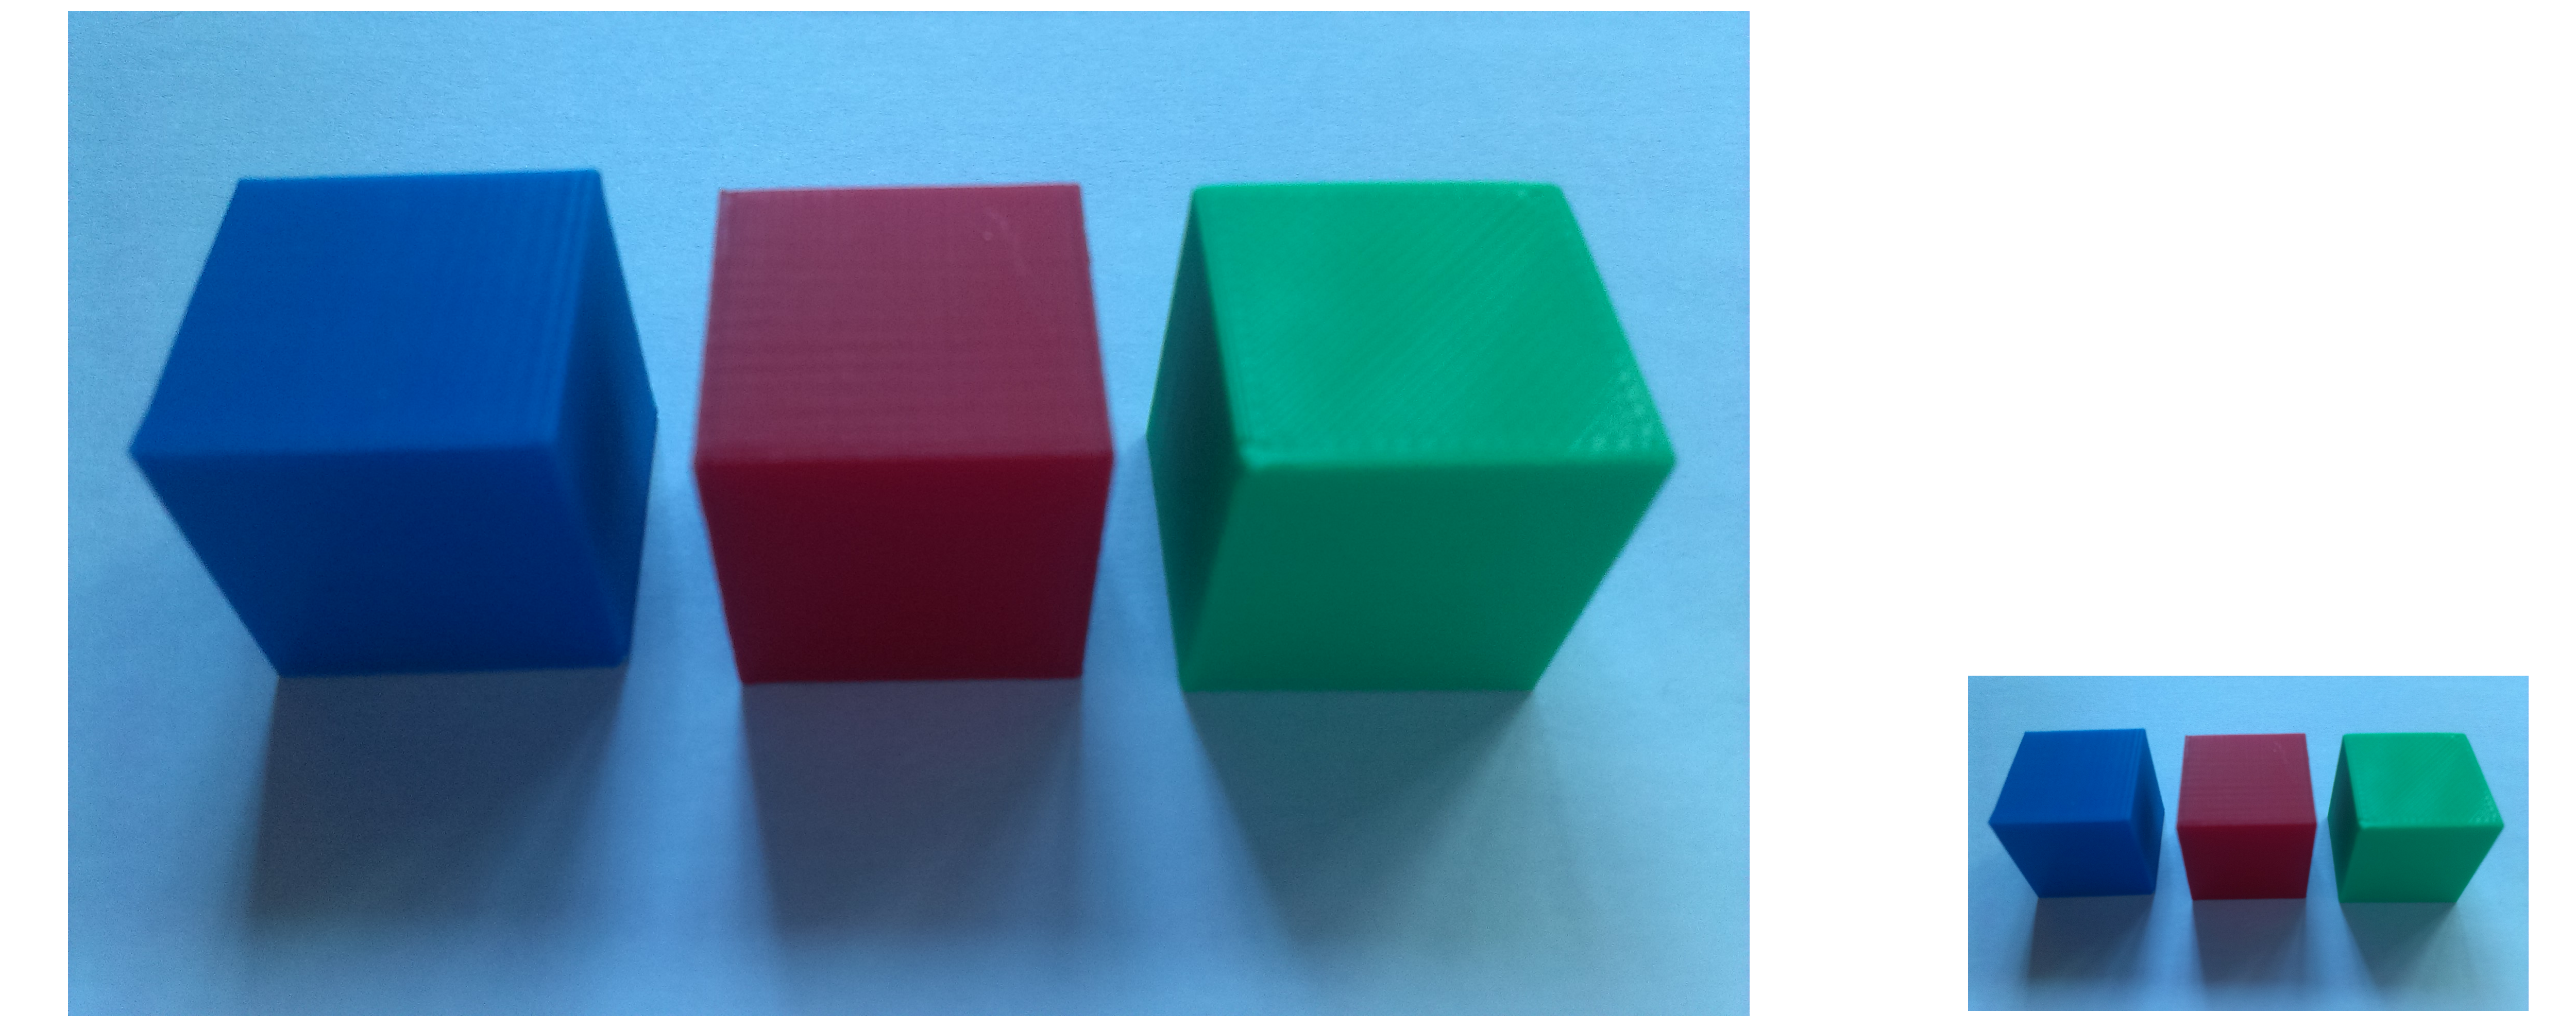
\includegraphics[width=0.6\textwidth]{img2}
  \caption{Comparación de tamaño entre imagen tomada con la cámara del teléfono y su reducción.}
\end{figure}

\noindent En definitiva, hay que tener en cuenta el tamaño que va a tener la imagen a tratar, ya que si es demasiado grande, tendremos que tener cuidado con el ruido, por lo que tendremos que aplicar técnicas de suavizado, y con imágenes demasiado pequeñas, puesto que podremos llegar a perder tanta información que el algoritmo no es capaz de reconocer nada.

\section{Segmentación}
Los primeros algoritmos de segmentación planteados fueron soluciones no demasiado buenas para la detección de los cuadrados, ya que únicamente me basaba en la característica del color de la imagen, obteniendo resultados en los que apenas se podían distinguir los cuadrados del resto del entorno.\\
Tras distintas pruebas, observé que el fondo negro era un discriminante magnífico para los colores, pero aun así, se mantenían ciertos problemas derivados del brillo. El color negro del fondo se modificó el pasado Jueves tras observar que el algoritmo trabajaba bien incluso con el fondo blanco, gracias a las imágenes que nos proporcionaba la cámara Logitec.\\
Otra decisión, fue establecer el color de los cuadrados con tonalidad mate, consiguiendo mitigar el brillo de los mismos.\\
Finalmente, decidimos incluir una nueva característica, la forma de los cuadrados, para conseguir distinguirlos del fondo.\\
El proceso de segmentación actual es el siguiente:

\begin{enumerate}
\item Aplicamos el algoritmo de \textit{Canny} para obtener los bordes de la imagen.
\begin{figure}[h!]
  \centering
      \includegraphics[width=0.5\textwidth]{img3}
  \caption{Bordes obtenidos por el algoritmo de Canny.}
\end{figure}

\item Se aplica una clausura, es decir, ``\textit{dilato}'' el píxel y luego lo ``\textit{adelgazo}'' (lo erosiono). Con esto conseguimos terminar de cerrar los contornos de los cuadrados, consiguiendo figuras totalmente cerradas.
\begin{figure}[h!]
  \centering
      \includegraphics[width=0.9\textwidth]{img4}
  \caption{Comparación entre la imagen con los bordes y la imagen tras aplicar la clausura.}
\end{figure}

\item Dada la imagen con los bordes cerrados, localizo los contornos.
\begin{figure}[h!]
  \centering
      \includegraphics[width=0.5\textwidth]{img5}
  \caption{Contornos localizados.}
\end{figure}

\item De todos los contornos, únicamente me quedo con los que se encuentran en el nivel 2 de profundidad.
\begin{figure}[h!]
  \centering
      \includegraphics[width=0.9\textwidth]{img10}
  \caption{Contornos de nivel 2.}
\end{figure}

\item Una vez tengo los contornos de los cuadrados, ya puedo moverme por ellos pudiendo seleccionar cualquiera de los cuadrados para conocer otra característica (en este caso, el color). Para poder empezar a moverme por ellos, les extraigo el fondo aplicando una imagen binaria (conocida como máscara) obtenida tras rellenar los contornos localizados en el paso anterior.
\begin{figure}[h!]
  \centering
      \includegraphics[width=0.9\textwidth]{img11}
  \caption{Imagen original a la que le aplico la máscara, obteniendo la separación de los objetos del fondo}
\end{figure}


\end{enumerate}
Finalmente, ya tenemos extraidos los cuadrados del fondo, terminando así, la fase de segmentación.

\section{Reconocimiento de los cuadrados}
Una vez tenemos los cuadrados localizados, lo único que tenemos que hacer es clasificarlos en alguna clase de color, es decir, decidir si son de color rojo, verde o azul. Para ello, recorremos todos los cuadrados, de tal forma que descomponemos la matriz RGB de cada uno de ellos en las tres componentes por separado.\\Una vez realizado el paso anterior, se calcula la media a cada una de las tres matrices obtenidas por cada cuadradito, observando cual de las tres medias es mayor para decidir si es de un color u otro.\\\\
El proceso explicado es el siguiente:
\begin{enumerate}
\item Seleccionamos un cuadrado.
\begin{figure}[h!]
  \centering
      \includegraphics[width=0.4\textwidth]{img_cd_rojo}
  \caption{Cuadrado seleccionado.}
\end{figure}
\newpage
\item Descomponemos en cada una de las componentes RGB.
\begin{figure}[h!]
  \centering
      \includegraphics[width=1\textwidth]{img_comp}
  \caption{Descomposición de la matriz original en cada una de sus componentes.}
\end{figure}

\item Se calcula la media de los píxeles para cada una de ellas.


\end{enumerate}

Una vez obtenidas las medias, se mira cual de ellas es la mayor, decidiendo así, si es de un color u otro.

\section{Actuación}
Llegados a este punto, ya somos capaces de coger un cuadrado y decir su color, ahora bien, ¿qué hacemos con esto?\\
En esta fase, se empieza a tener contacto con la Arduino para poder realizar las distintas acciones posibles, es decir, mover la cintura o alguno de los dos brazos.\\
A día de hoy, se ha logrado mover la cintura según el ángulo de giro hacia un cuadrado. Para ello, se siguen los siguientes pasos:

\begin{enumerate}
\item Se selecciona un cuadrado según su color en el orden establecido.
\item Se calcula su punto central.
\begin{figure}[h!]
  \centering
      \includegraphics[width=0.4\textwidth]{img12}
  \caption{Punto central cuadrado.}
\end{figure}
\newpage

\item Se calcula la recta que divide la imagen en dos y la recta que va desde el punto inferior de la recta anterior hasta el punto calculado.
\begin{figure}[h!]
  \centering
      \includegraphics[width=0.4\textwidth]{img13}
  \caption{Rectas.}
\end{figure}

\item Se calculan los vectores directores necesarios para obtener el ángulo de giro para la cadera del robot.

\item Por último, se le envía a la Arduino los siguientes datos:
	\begin{itemize}
	\item La acción. En este caso un 1 para indicar que se va a mover la cadera.
	\item El movimiento. Si va a ser para la izquierda (un 1) o para la derecha (un 2).
	\item Se calculan el número de dígitos que tiene el ángulo de giro. Esto se realiza para indicarle a la Arduino que los siguientes \textit{x} valores que reciba son el ángulo.
	\item El ángulo. Que se enviará dígito a dígito por el puerto serie.
	\end{itemize}

\end{enumerate}

\section{Explicación algoritmo Arduino}
En esta sección, voy a explicar el planteamiento del algoritmo que se va a usar para la placa arduino.\\\\
En un principio, la Arduino escucha por el puerto serie a la espera de que le llegue información, siendo el 0 el valor que se lee por el \textit{Serial}. Para eliminar dichos 0, se mantiene una espera ocupada eliminando todo valor del Serial que sea menor o igual que 0.\\
Cuando se detecta que llega algo de información se comprueba que dígito es; si el dígito es un 1, se entiende que se va a recibir información referente a la cadera; si es un 2, será información para mover el brazo derecho; si es un 3, será para el brazo izquierdo.\\
Una vez sabemos que es lo que vamos a mover, se vuelve a realizar una espera ocupada para eliminar aquel ruido que se haya podido colar en el Serial a la espera de otro valor. En cuanto llega información, dependiendo de lo que se vaya a mover, se realizará un movimiento u otro. Como ahora mismo lo único que se ha programado para moverse es la cadera, continuaré la explicación como si fuese a moverla.\\
La información que nos llega en este caso, se comprueba para saber si nos vamos a mover para la derecha o para la izquierda y, sabiendo esto, que ángulo tengo que girar.\\
Para obtener el ángulo se emplea una solución software para juntar las cifras individuales que llegan por el Serial.\\
Finalmente, se realiza una regla de tres para saber el número de pasos que debe dar el motor paso a paso para colocarse en el ángulo calculado.

\section{Conclusión}
Al comienzo de este proyecto, podía observar una clara distinción entre la informática y lo industrial, puesto que me he dedicado a lo que sería la lógica del robot, abstrayéndome de la electrónica, electricidad y mecánica que existe en un proyecto como este. Tras el paso de las semanas, y en concreto, las acciones y decisiones tomadas a lo largo de estas últimas semanas; como elegir la altura del robot, la colocación de los servos para tener un poco más de altura en los brazos para que no estén tan caídos, la posición de la cámara, etc, me han ayudado a aprender que existen conceptos determinantes, como es el peso, que hay que tener en cuenta en el diseño de piezas y materiales que se vayan a utilizar en el proyecto.\\
En cuanto a la parte electrónica, que es con la que más tiempo he estado, se necesitan conocer los conceptos que acabamos de mencionar, ya que en base a ellos, se eligirá unos elementos u otros, ya sea un motor o servo más potente o, simplemente, si el voltaje y la intensidad que pasan por un componente son suficientes para que este funcione correctamente o muestre problemas al realizar alguna acción derivada de estos dos aspectos.\\
Respecto a la programación de la Arduino, al principio existía la molestia del procedimiento \textbf{loop()}, ya que funciona igual que un bucle que itera de forma indefinida. Tras acostumbrarme a este hecho, la programación no ha sido más complicada que escribir un programa sencillo en C/C++. Una de las cosas que más me ha gustado en este proyecto es que ha sido fascinante ver como un programa, al que estamos acostumbrados a que nos muestre un resultado por la salida estándar del ordenador, sea capaz de llegar de encender un diodo led o, incluso, mover un motor.\\
En definitiva, lo que quería decir con todo lo anterior, es que las distintas especialidades o tecnologías, como se quiera ver, son distintas pero se necesitan unas a otras para lograr llevar a buen puerto un proyecto industrial como este.

\end{document}
